\section{Практика 10. Максимальный поток}

\subsection{Практика}

\begin{itemize}

  \item Найти паросочетание в двудольном графе, используя максимальный поток.

  \item Недавно сотрудники отдела купили себе большой набор чайных пакетиков, 
который содержит $a_1$ пакетиков чая сорта номер 1, $a_2$ пакетиков чая сорта 
номер 2, ..., $a_m$ пакетиков чая сорта номер $m$. Теперь они хотят знать, на 
какое максимальное число дней им может хватить купленного набора так, чтобы в 
каждый из дней каждому из сотрудников доставался пакетик чая одного из его 
любимых сортов.

  \item Дан ориентированный граф $G = \langle V, E \rangle$ без циклов с 
одним стоком $t$ и одним истоком $s$. Каждое ребро имеет пропускную способность
$c_e$. Блокирующим потоком назовем поток $f : E \rightarrow \mathbb{R}$ такой, 
что
\begin{enumerate}
  \item для любой вершины, кроме стока и истока, суммарный поток равен нулю;
  \item для каждого ребра $e$ выполняется $f_e \leq c_e$;
  \item на любом пути от истока к стоку найдется насыщенное ребро ($c_e = f_e$).
\end{enumerate}
  Найдите блокирующий поток за $O(VE)$.

\end{itemize}

\subsection{Домашнее задание. Практика}
\textbf{Дедлайн: 4 мая 23.59}

\begin{enumerate}

  \item Сдать \href{http://acm.timus.ru/problem.aspx?space=1&num=1449}{Тимус 1449}.

  \item Сдать \href{http://contest2.yandex.ru/contest/511/enter/}{Яндекс.Контест}. 
Джеллейные кошки сдавать по желанию.

\end{enumerate}

\subsection{Домашнее задание. Теория}
\textbf{Дедлайн: 23 апреля, 23.59}
\begin{enumerate}

  \item В турнире участвуют $n$ команд. Каждая команда играет с каждой ровно
один раз. Каждый матч завершается победой одной из команд. За победу команде
дается одно очко, за поражение -- ноль. Чемпионом становится команда, у которой
количество очков больше всех.

  Прошло несколько матчей, и известны их результаты. Требуется определить, может
ли первая команда стать чемпионом. Задачу свести к потоку. Сеть может иметь
$O(n^2)$ вершин.

  \item Дана прямоугольная сетка $n \times m$. Некоторые узлы сетки выделены. 
Для каждого выделенного узла требуется проложить путь по ребрам сети на границу, 
так чтобы никакие два пути вершинно не пересекались (см. рисунок). 
Задачу свести к потоку. Размер сети должен быть пропорционален $n \times m$.

  \begin{center}
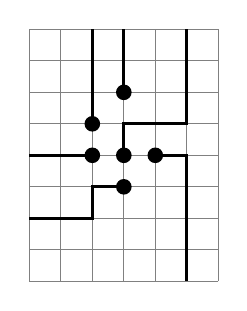
\begin{tikzpicture}[ thick, every node/.style={scale=1},level distance=1.7cm, sibling distance=2cm]

  \draw[step=0.4cm,thin, gray] (0, 0) grid (2.4, 3.2);

  \node[circle, fill=black, inner sep=0.7mm] at (1.2, 1.2) {};
  \draw[very thick] (1.2, 1.2) -- (0.8, 1.2) -- (0.8, 0.8) -- (0.0, 0.8);

  \node[circle, fill=black, inner sep=0.7mm] at (0.8, 1.6) {};
  \draw[very thick] (0.8, 1.6) -- (0.4, 1.6) -- (0.0, 1.6);

  \node[circle, fill=black, inner sep=0.7mm] at (1.6, 1.6) {};
  \draw[very thick] (1.6, 1.6) -- (2.0, 1.6) --  (2.0, 0);

  \node[circle, fill=black, inner sep=0.7mm] at (1.2, 2.4) {};
  \draw[very thick] (1.2, 2.4) -- (1.2, 3.2);

  \node[circle, fill=black, inner sep=0.7mm] at (0.8, 2) {};
  \draw[very thick] (0.8, 2) -- (0.8, 3.2);

  \node[circle, fill=black, inner sep=0.7mm] at (1.2, 1.6) {};
  \draw[very thick] (1.2, 1.6) -- (1.2, 2) -- (2, 2) -- (2, 3.2);



\end{tikzpicture}
\end{center}
    

  \item Дана сеть $G = \langle V, E, c, s, t \rangle$, где $c$ -- пропускные 
способности ребер, $s$ и $t$ -- исток и сток соответственно. Посмотрим на 
следующий алгоритм поиска максимального потока. Пусть начальный поток $f$ равен 
нулю.
\begin{enumerate}
  \item Сформируем остаточную сеть $R_f = \langle V, E_f, c_f \rangle$ на основе 
    текущего потока.
  \item Запустим из вершины $s$ BFS и найдем реберное расстояние 
$\texttt{dist(v)}$ от вершины $s$ до каждой.
  \item Построим дополнительную сеть $F = \langle V, E_F, c_f \rangle$.
  Ребро $(u, v)$ входит в сеть $F$ тогда и только тогда, когда оно входит в текущую
  остаточную сеть $R$ и $\texttt{dist(v)} - \texttt{dist(u)} = 1$.
  \item Найдем блокирующий поток в сети $F$ и добавим его к текущему ответу. 
    Вернемся к пункту 1.
\end{enumerate}
  Докажите, что после каждой итерации поиска блокирующего потока расстояние между
  стоком и истоком увеличивается хотя бы на единицу.


\end{enumerate}



\clearpage
